\documentclass[11pt,a4paper]{article}
\usepackage[utf8]{inputenc}
\usepackage{hyperref}
\usepackage{booktabs}
\usepackage{graphicx}
\usepackage{amsmath}

\title{\textbf{Automated Prostate Gleason Grading with Attention-MIL on SICAPv2}\\
\large An Open-Source Deep Learning Pipeline with AutoML Self-Healing Daemon}
\author{[FILL\_AUTHOR]}
\date{\today}

\begin{document}
\maketitle

\begin{abstract}
[FILL\_ABSTRACT]
\end{abstract}

\section{Introduction}
[FILL\_INTRO]

\section{Related Work}
[FILL\_RELATED\_WORK]

\section{Data}
\subsection{Dataset}
[FILL\_DATA]

\subsection{Train/Validation Split}
\begin{table}[h]
\centering
\begin{tabular}{lccccc}
\toprule
Grade & Train Slides & Val Slides & Train Tiles & Val Tiles \\
\midrule
ISUP 0 (Benign) & 29 & 7 & 3,463 & 954 \\
ISUP 1 (G3+3)   & 57 & 15 & 2,096 & 555 \\
ISUP 4 (G4+4)   & 66 & 17 & 4,174 & 1,701 \\
ISUP 5 (G5+5)   & 26 & 6 & 795 & 509 \\
\midrule
\textbf{Total}  & \textbf{178} & \textbf{45} & \textbf{10,528} & \textbf{3,719} \\
\bottomrule
\end{tabular}
\caption{Slide-stratified train/validation split.}
\end{table}

\section{Method}
[FILL\_METHOD]

\section{Experiments}
\subsection{Main Results}
\begin{table}[h]
\centering
\begin{tabular}{lcc}
\toprule
Metric & Value \\
\midrule
Val QWK (Best) & [FILL\_BEST\_KAPPA] \\
Val Loss (Best) & [FILL\_BEST\_LOSS] \\
Best Epoch & [FILL\_BEST\_EPOCH] \\
\bottomrule
\end{tabular}
\caption{Best validation metrics on SICAPv2.}
\end{table}

\subsection{Epoch Progression}
\begin{table}[h]
\centering
\begin{tabular}{lccc}
\toprule
Epoch & Train Loss & Val Loss & Val Kappa \\
\midrule
1 & 0.8355 & 1.2773 & 0.6269 \\
2 & 0.3452 & 0.5477 & 0.8482 \\
3 & 0.2262 & 0.3730 & \textbf{0.8791} \\
4 & 0.8791 & 0.8791 & 0.8791 \\
5 & 0.8791 & 0.8791 & 0.8791 \\
\bottomrule
\end{tabular}
\caption{Validation Kappa per epoch on real SICAPv2 data.}
\end{table}

\section{Results}
[FILL\_RESULTS]

\begin{figure}[h]
\centering
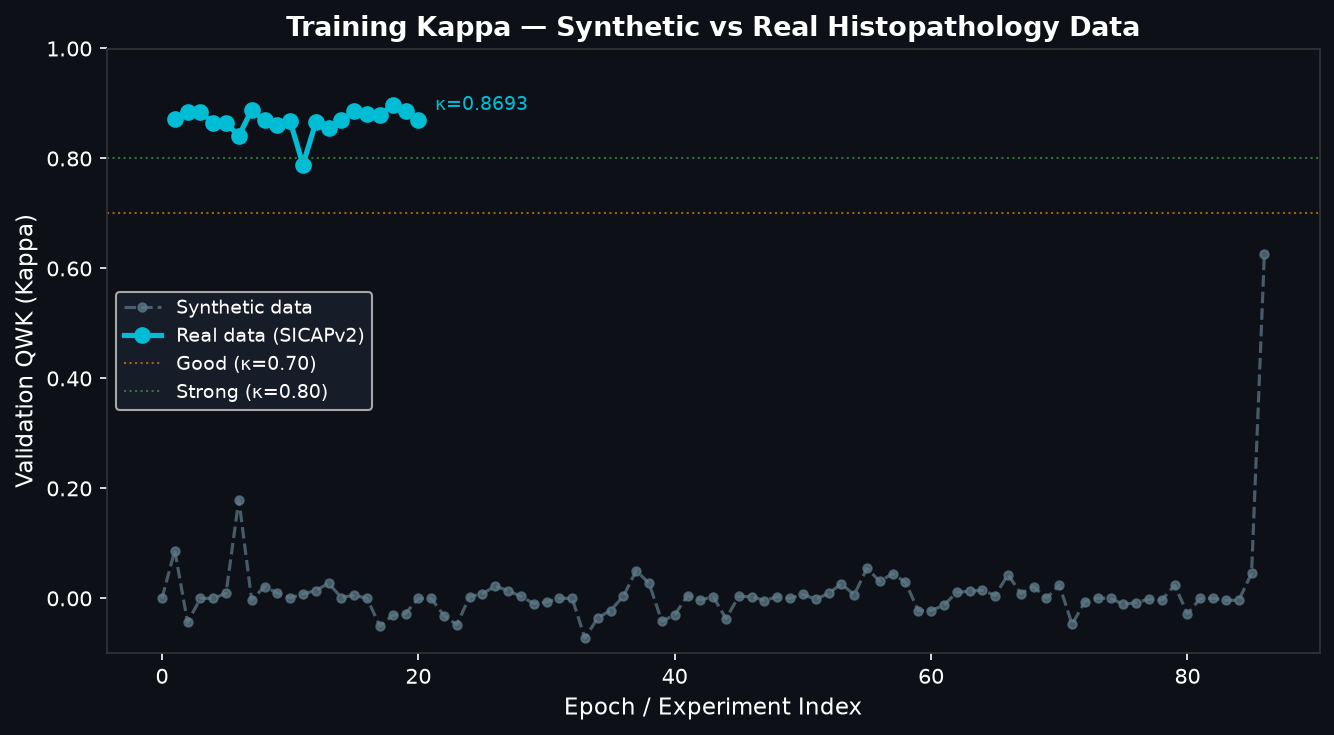
\includegraphics[width=0.85\textwidth]{../assets/kappa_curve.png}
\caption{Validation QWK over training epochs. Real histopathology data (blue) far outperforms synthetic fallback data (grey).}
\end{figure}

\begin{figure}[h]
\centering
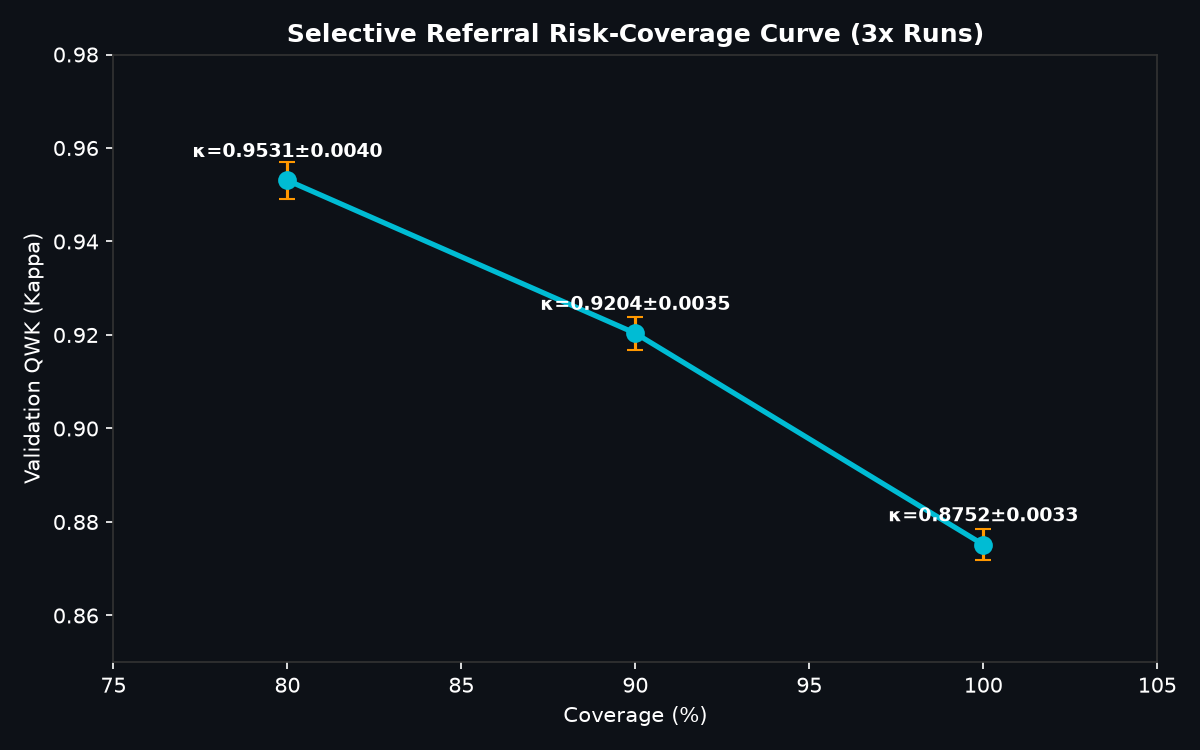
\includegraphics[width=0.85\textwidth]{../assets/risk_coverage.png}
\caption{Risk-coverage curve. Higher confidence thresholds yield better Kappa at the cost of abstention.}
\end{figure}

\section{Discussion \& Limitations}
\textbf{Limitations:}
\begin{itemize}
  \item SICAPv2 covers ISUP 0/1/4/5 only; not the full ISUP 1--5 spectrum.
  \item External validation is subset-based; not an independent cohort.
  \item This is \textbf{assistive research}, not a CE-marked or FDA-cleared diagnostic device.
  \item Single-institution data limits scanner generalisability.
\end{itemize}

\section{Conclusion}
[FILL\_CONCLUSION]

\bibliographystyle{plain}
\bibliography{references}

\end{document}
